% Appendix C: Extended Results

\section{Correlation Matrix}

Correlation matrix for relevant features of both benchmarks.

\begin{figure}[h]
\centering
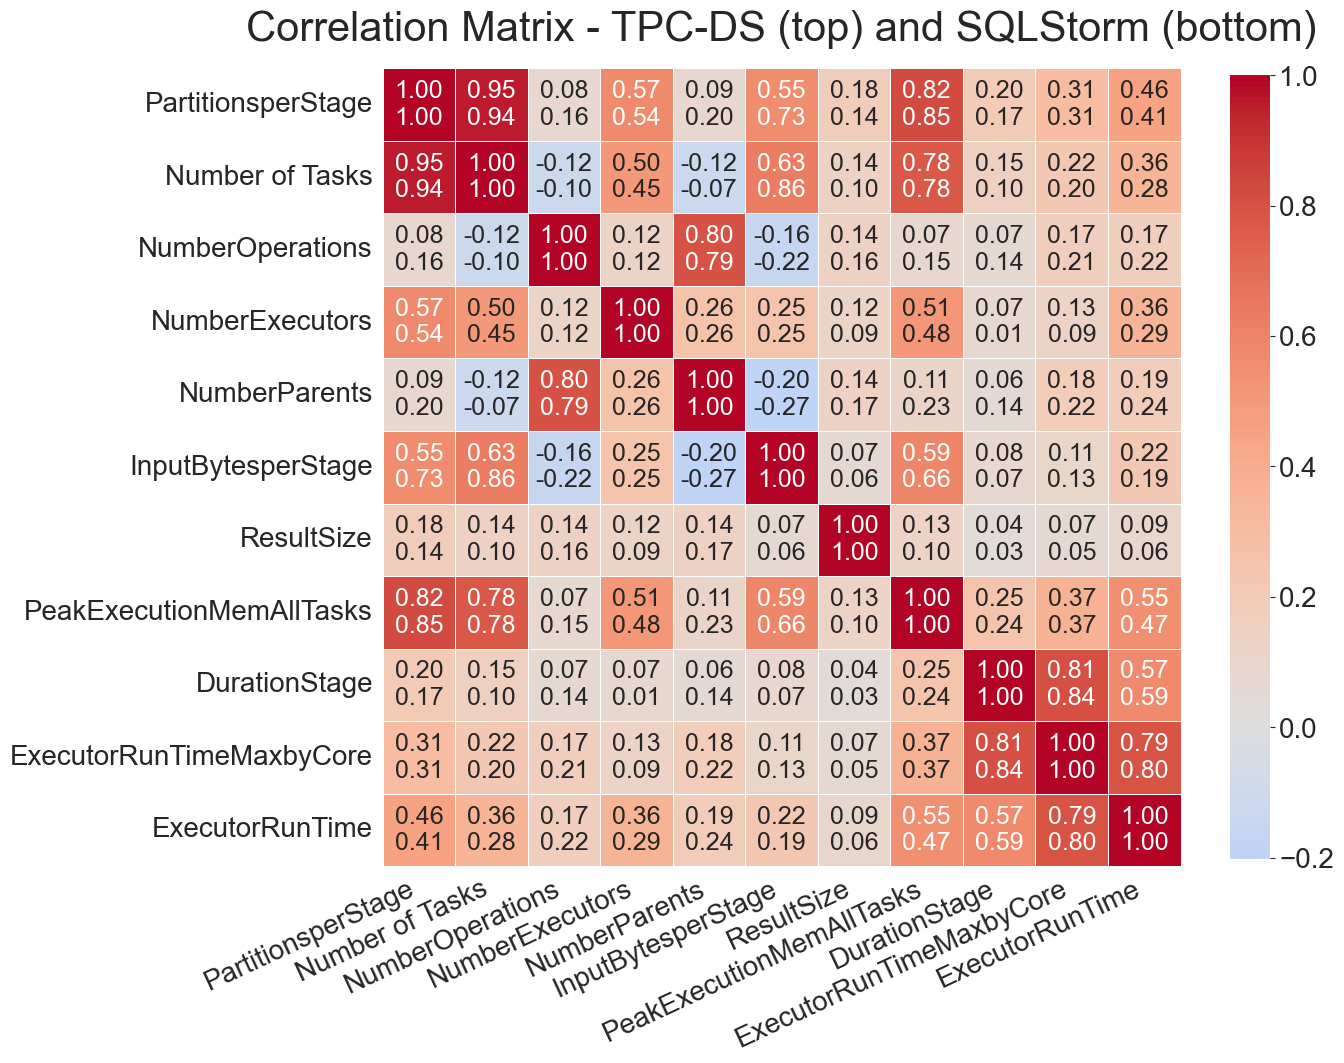
\includegraphics[width=\textwidth]{figs/correlation-matrix.png}
\caption{TPC-DS and SQLStorm Correlation Matrix}
\label{fig:correlation-matrix}
\end{figure}

\section{SHAP Plots Our Models}

SHAP plots for our cost prediction models for both benchmarks.

\subsection{TPC-DS}

\subsubsection{0-shot model}

\begin{figure}[h]
\centering
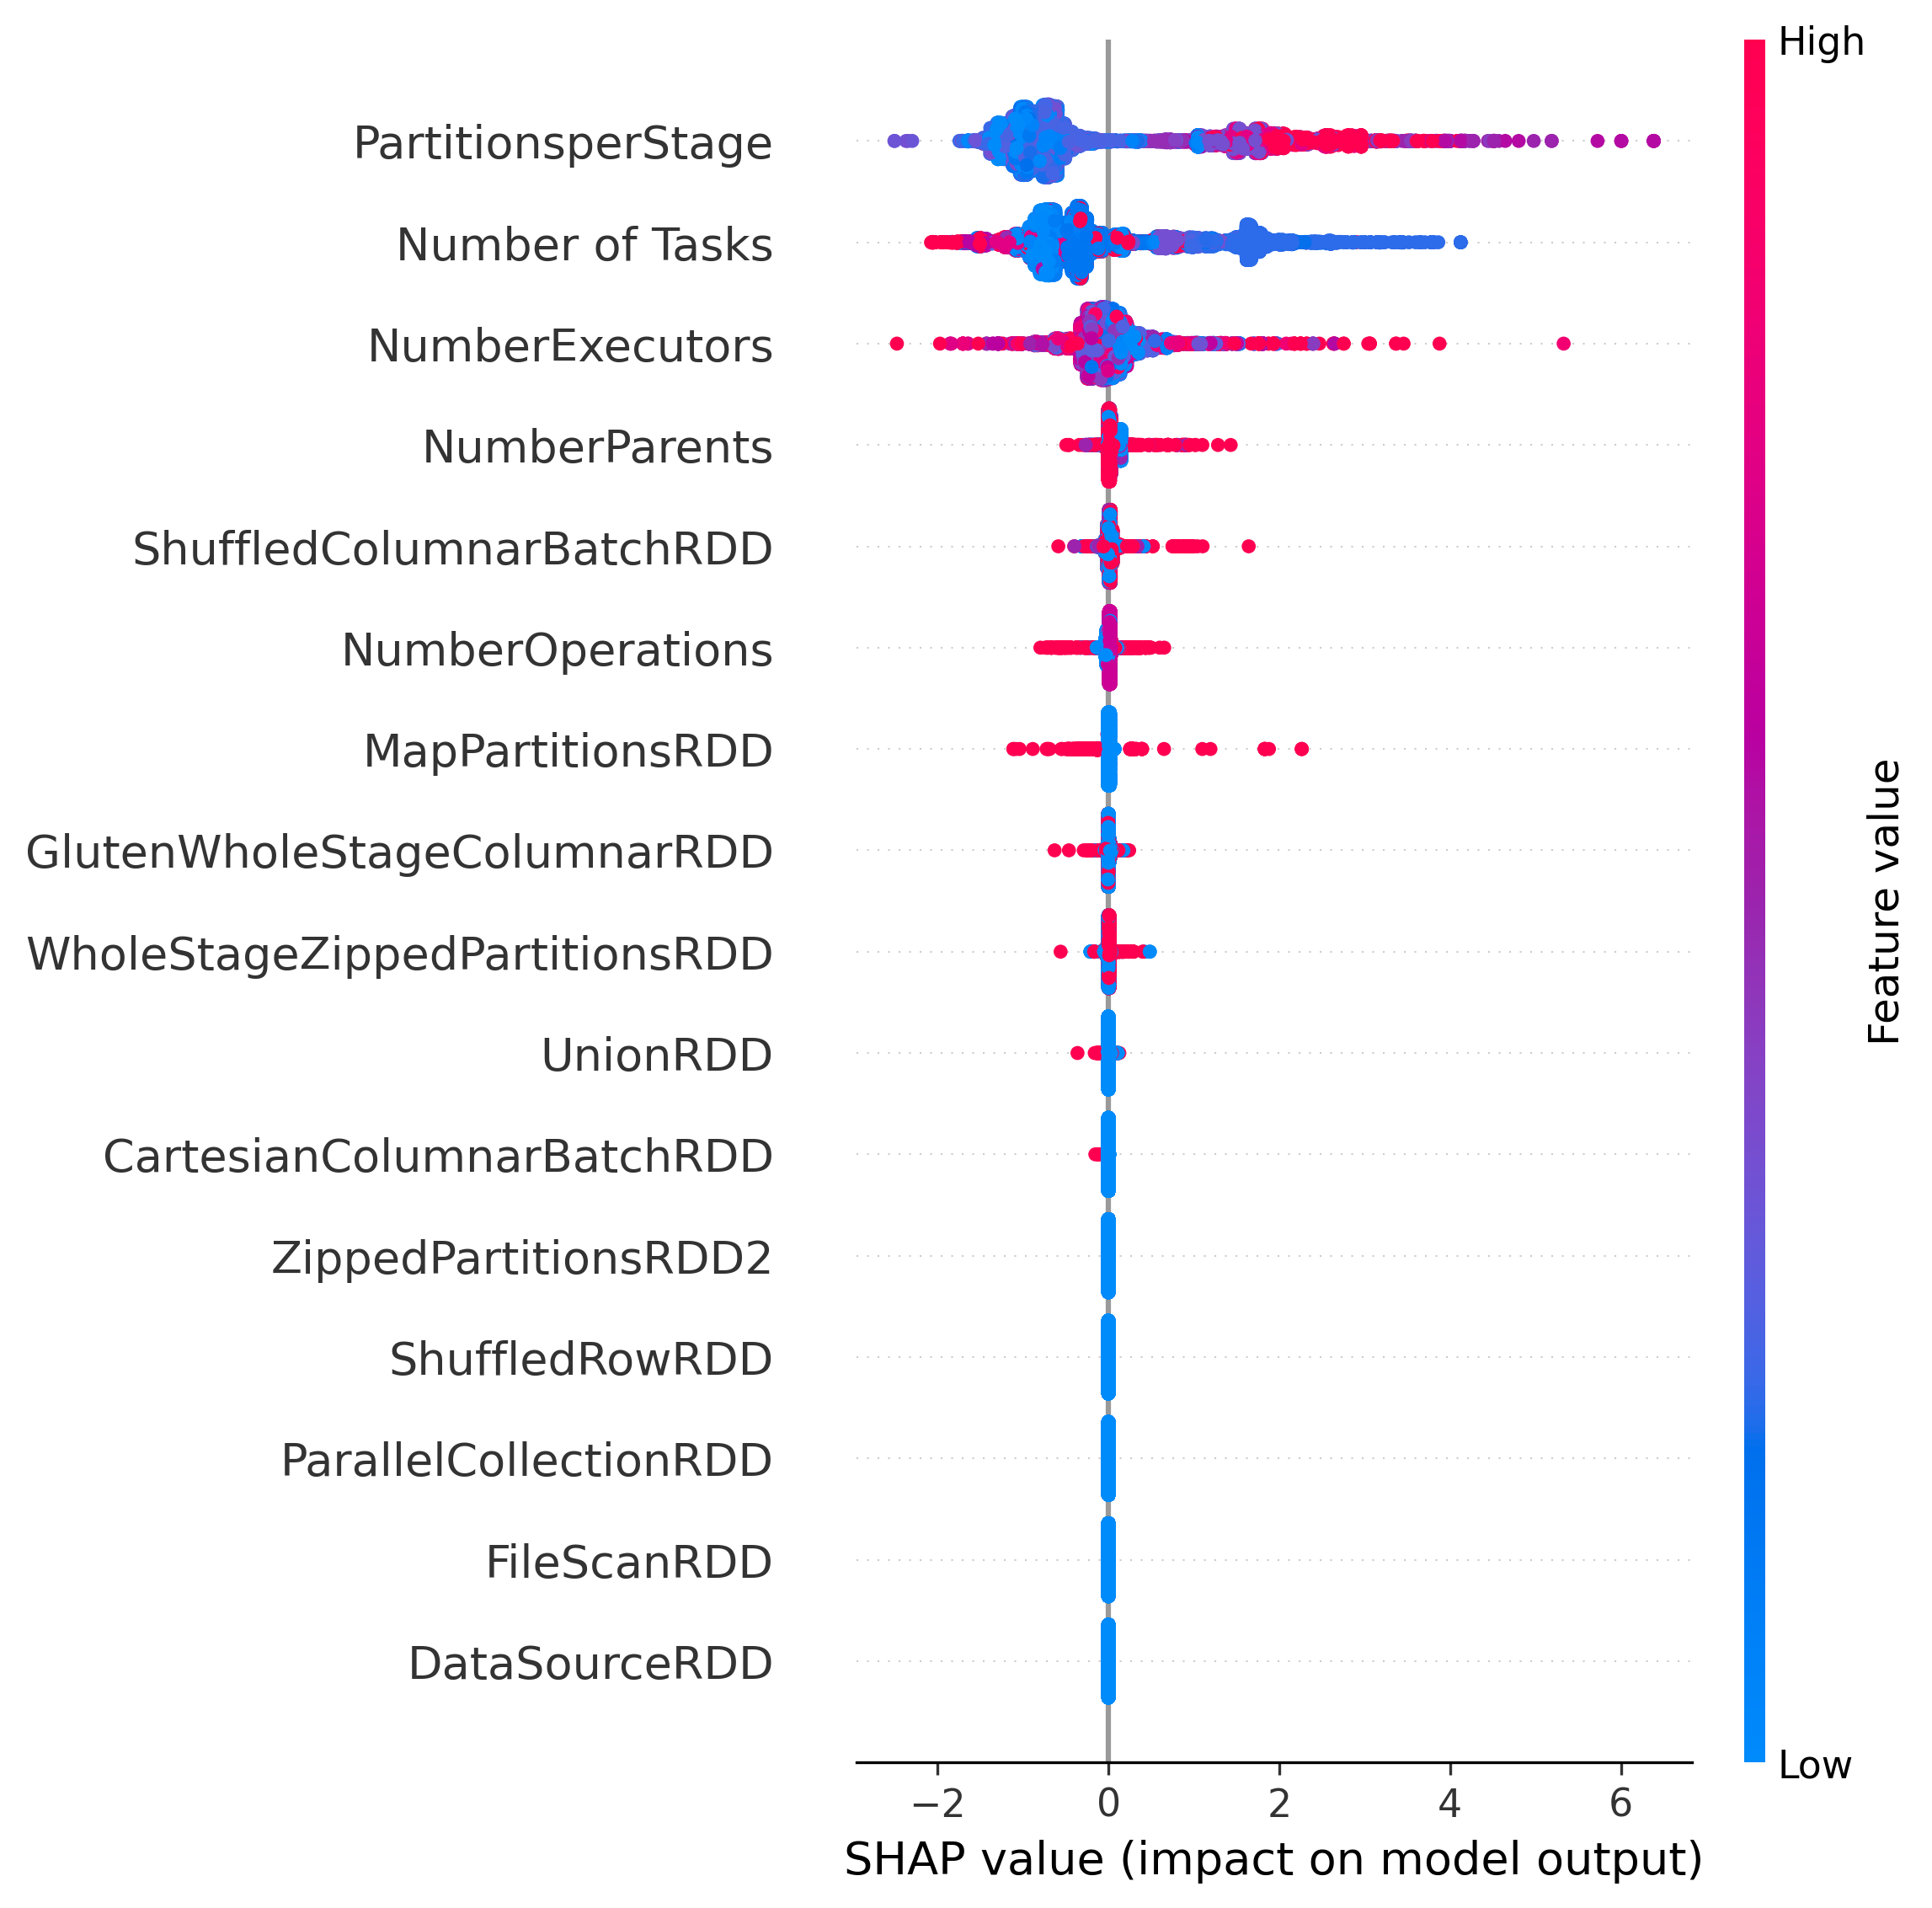
\includegraphics[width=\textwidth]{figs/predictor_shap_beeswarm_tpcds_ExecutorRunTimeMaxbyCore_log-True_online.png}
\caption{TPC-DS SHAP Plot 0-shot Cost Predictor}
\label{fig:tpcds-shap-0shot}
\end{figure}

\subsubsection{n-shot model}

\begin{figure}[h]
\centering
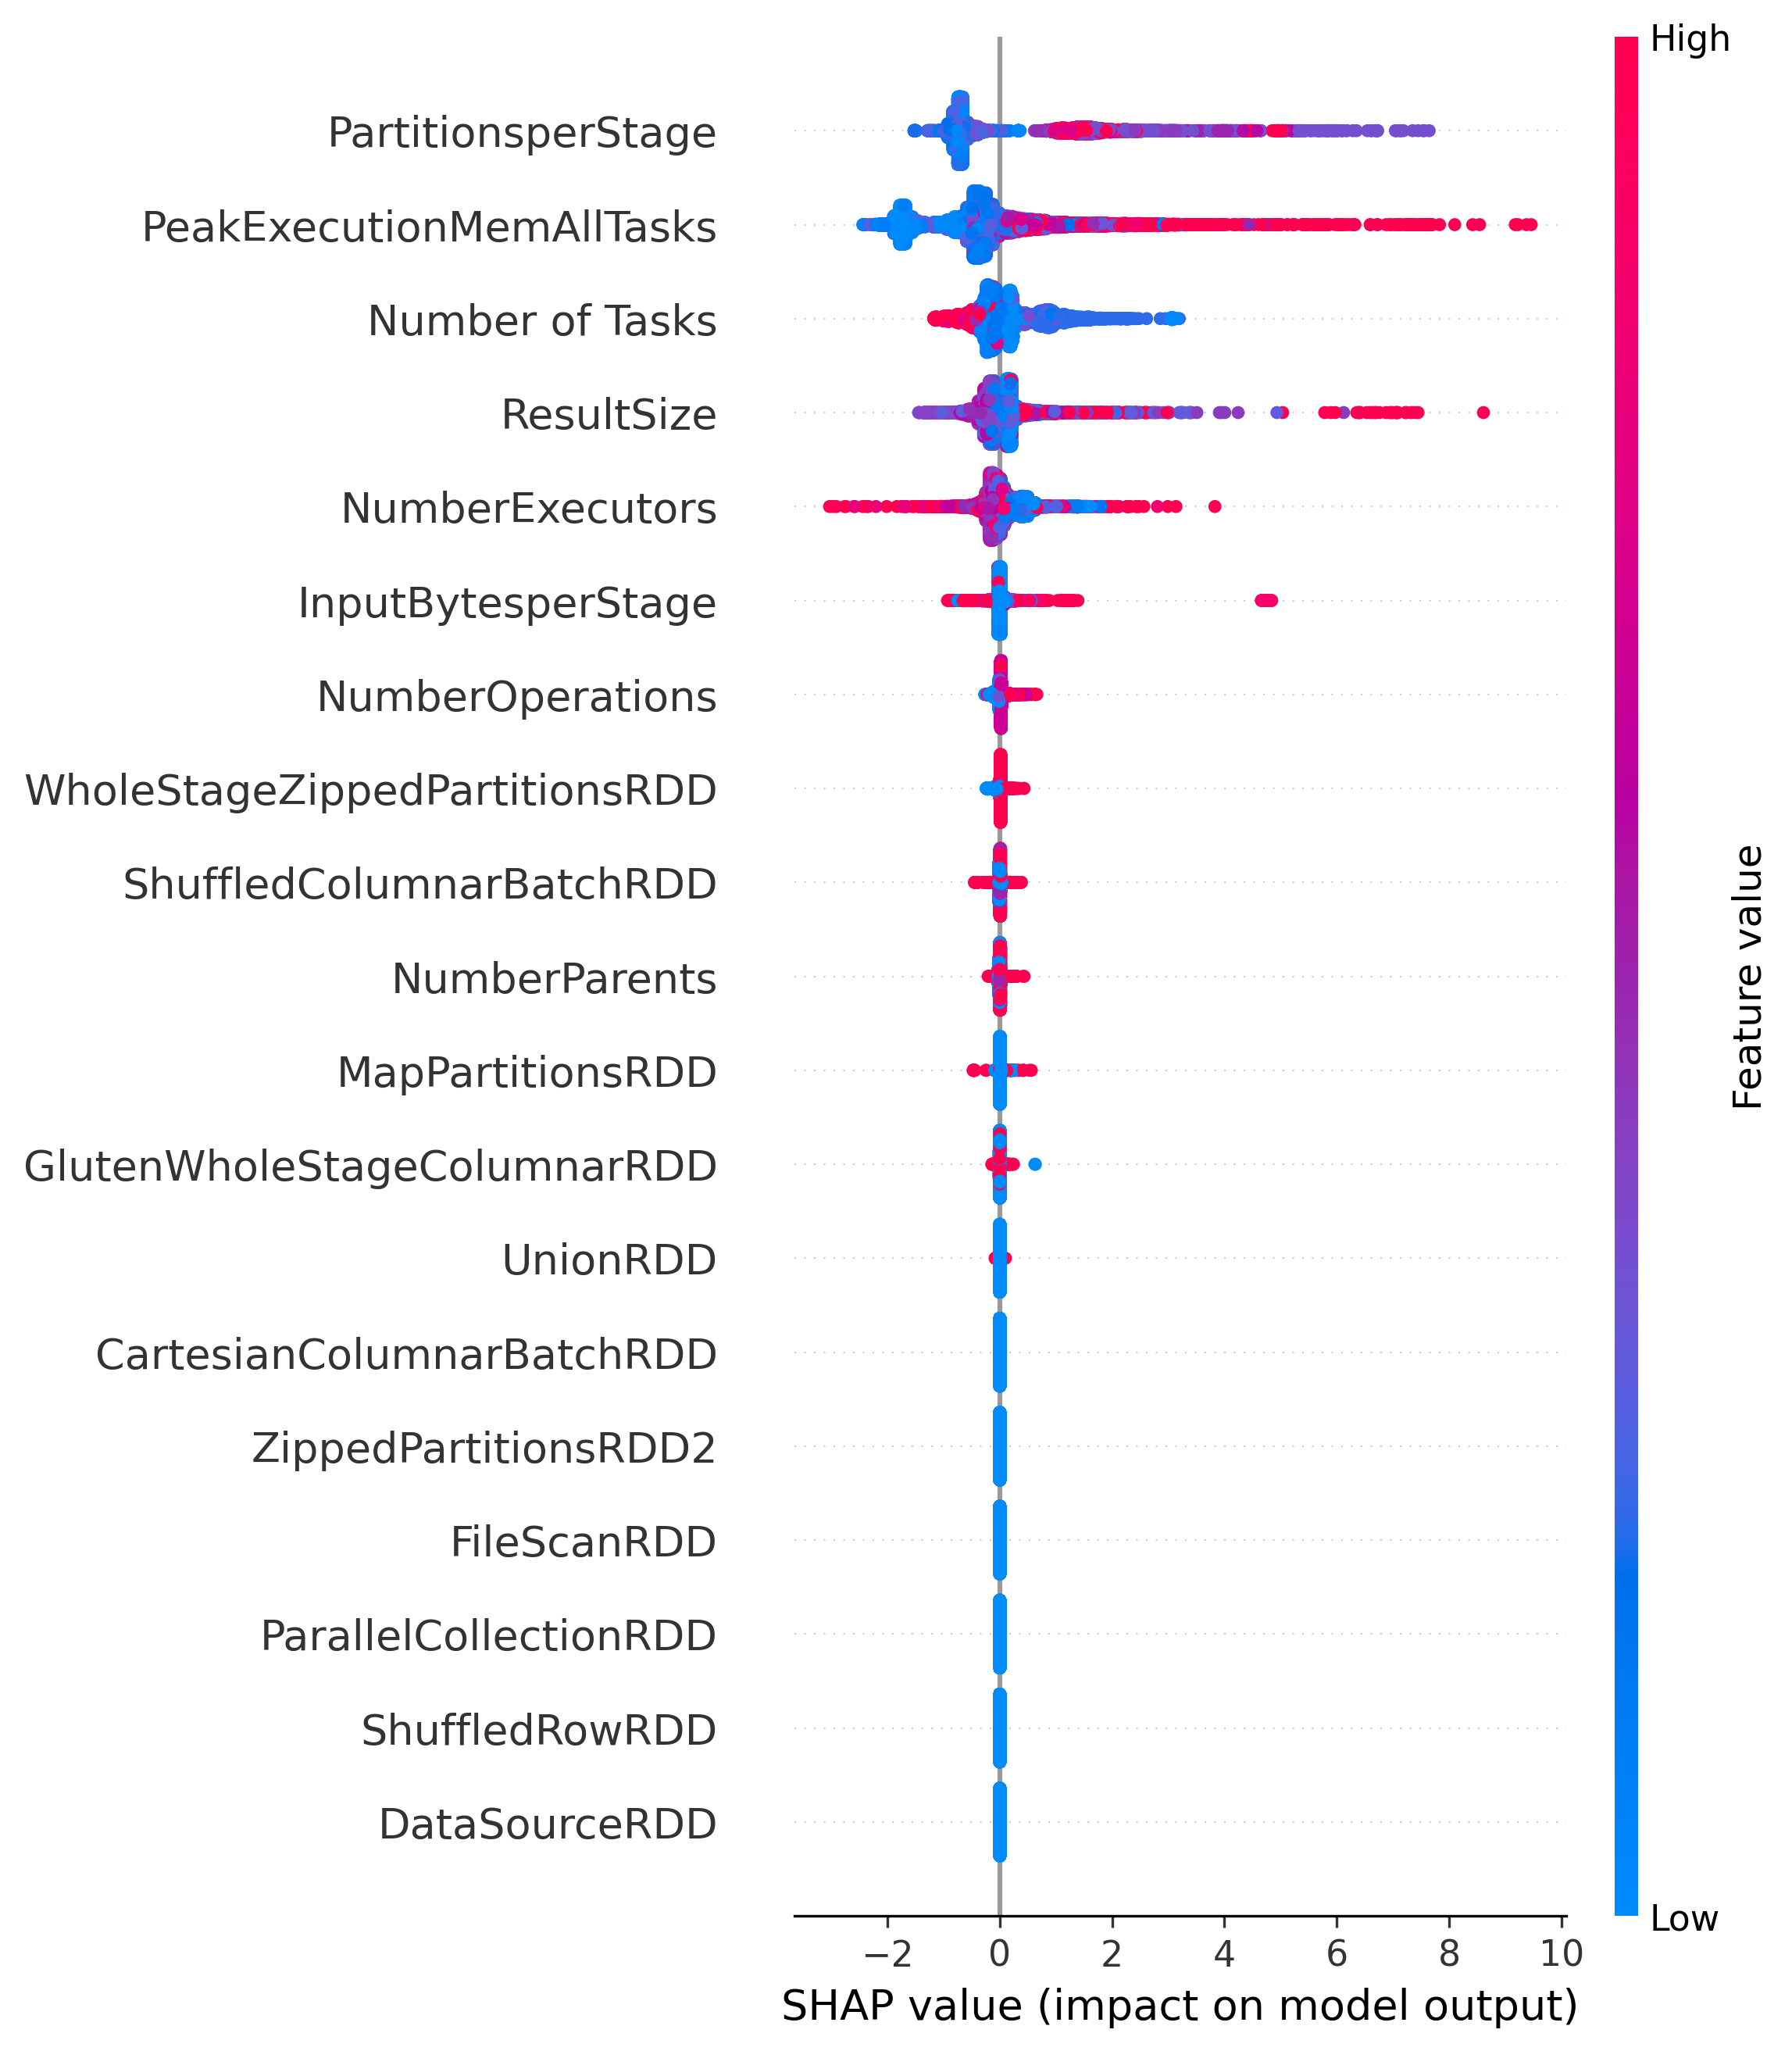
\includegraphics[width=\textwidth]{figs/predictor_shap_beeswarm_tpcds_ExecutorRunTimeMaxbyCore_log-True_offline.png}
\caption{TPC-DS SHAP Plot n-shot Cost Predictor}
\label{fig:tpcds-shap-nshot}
\end{figure}

\subsection{SQLStorm}

\subsubsection{0-shot model}

\begin{figure}[h]
\centering
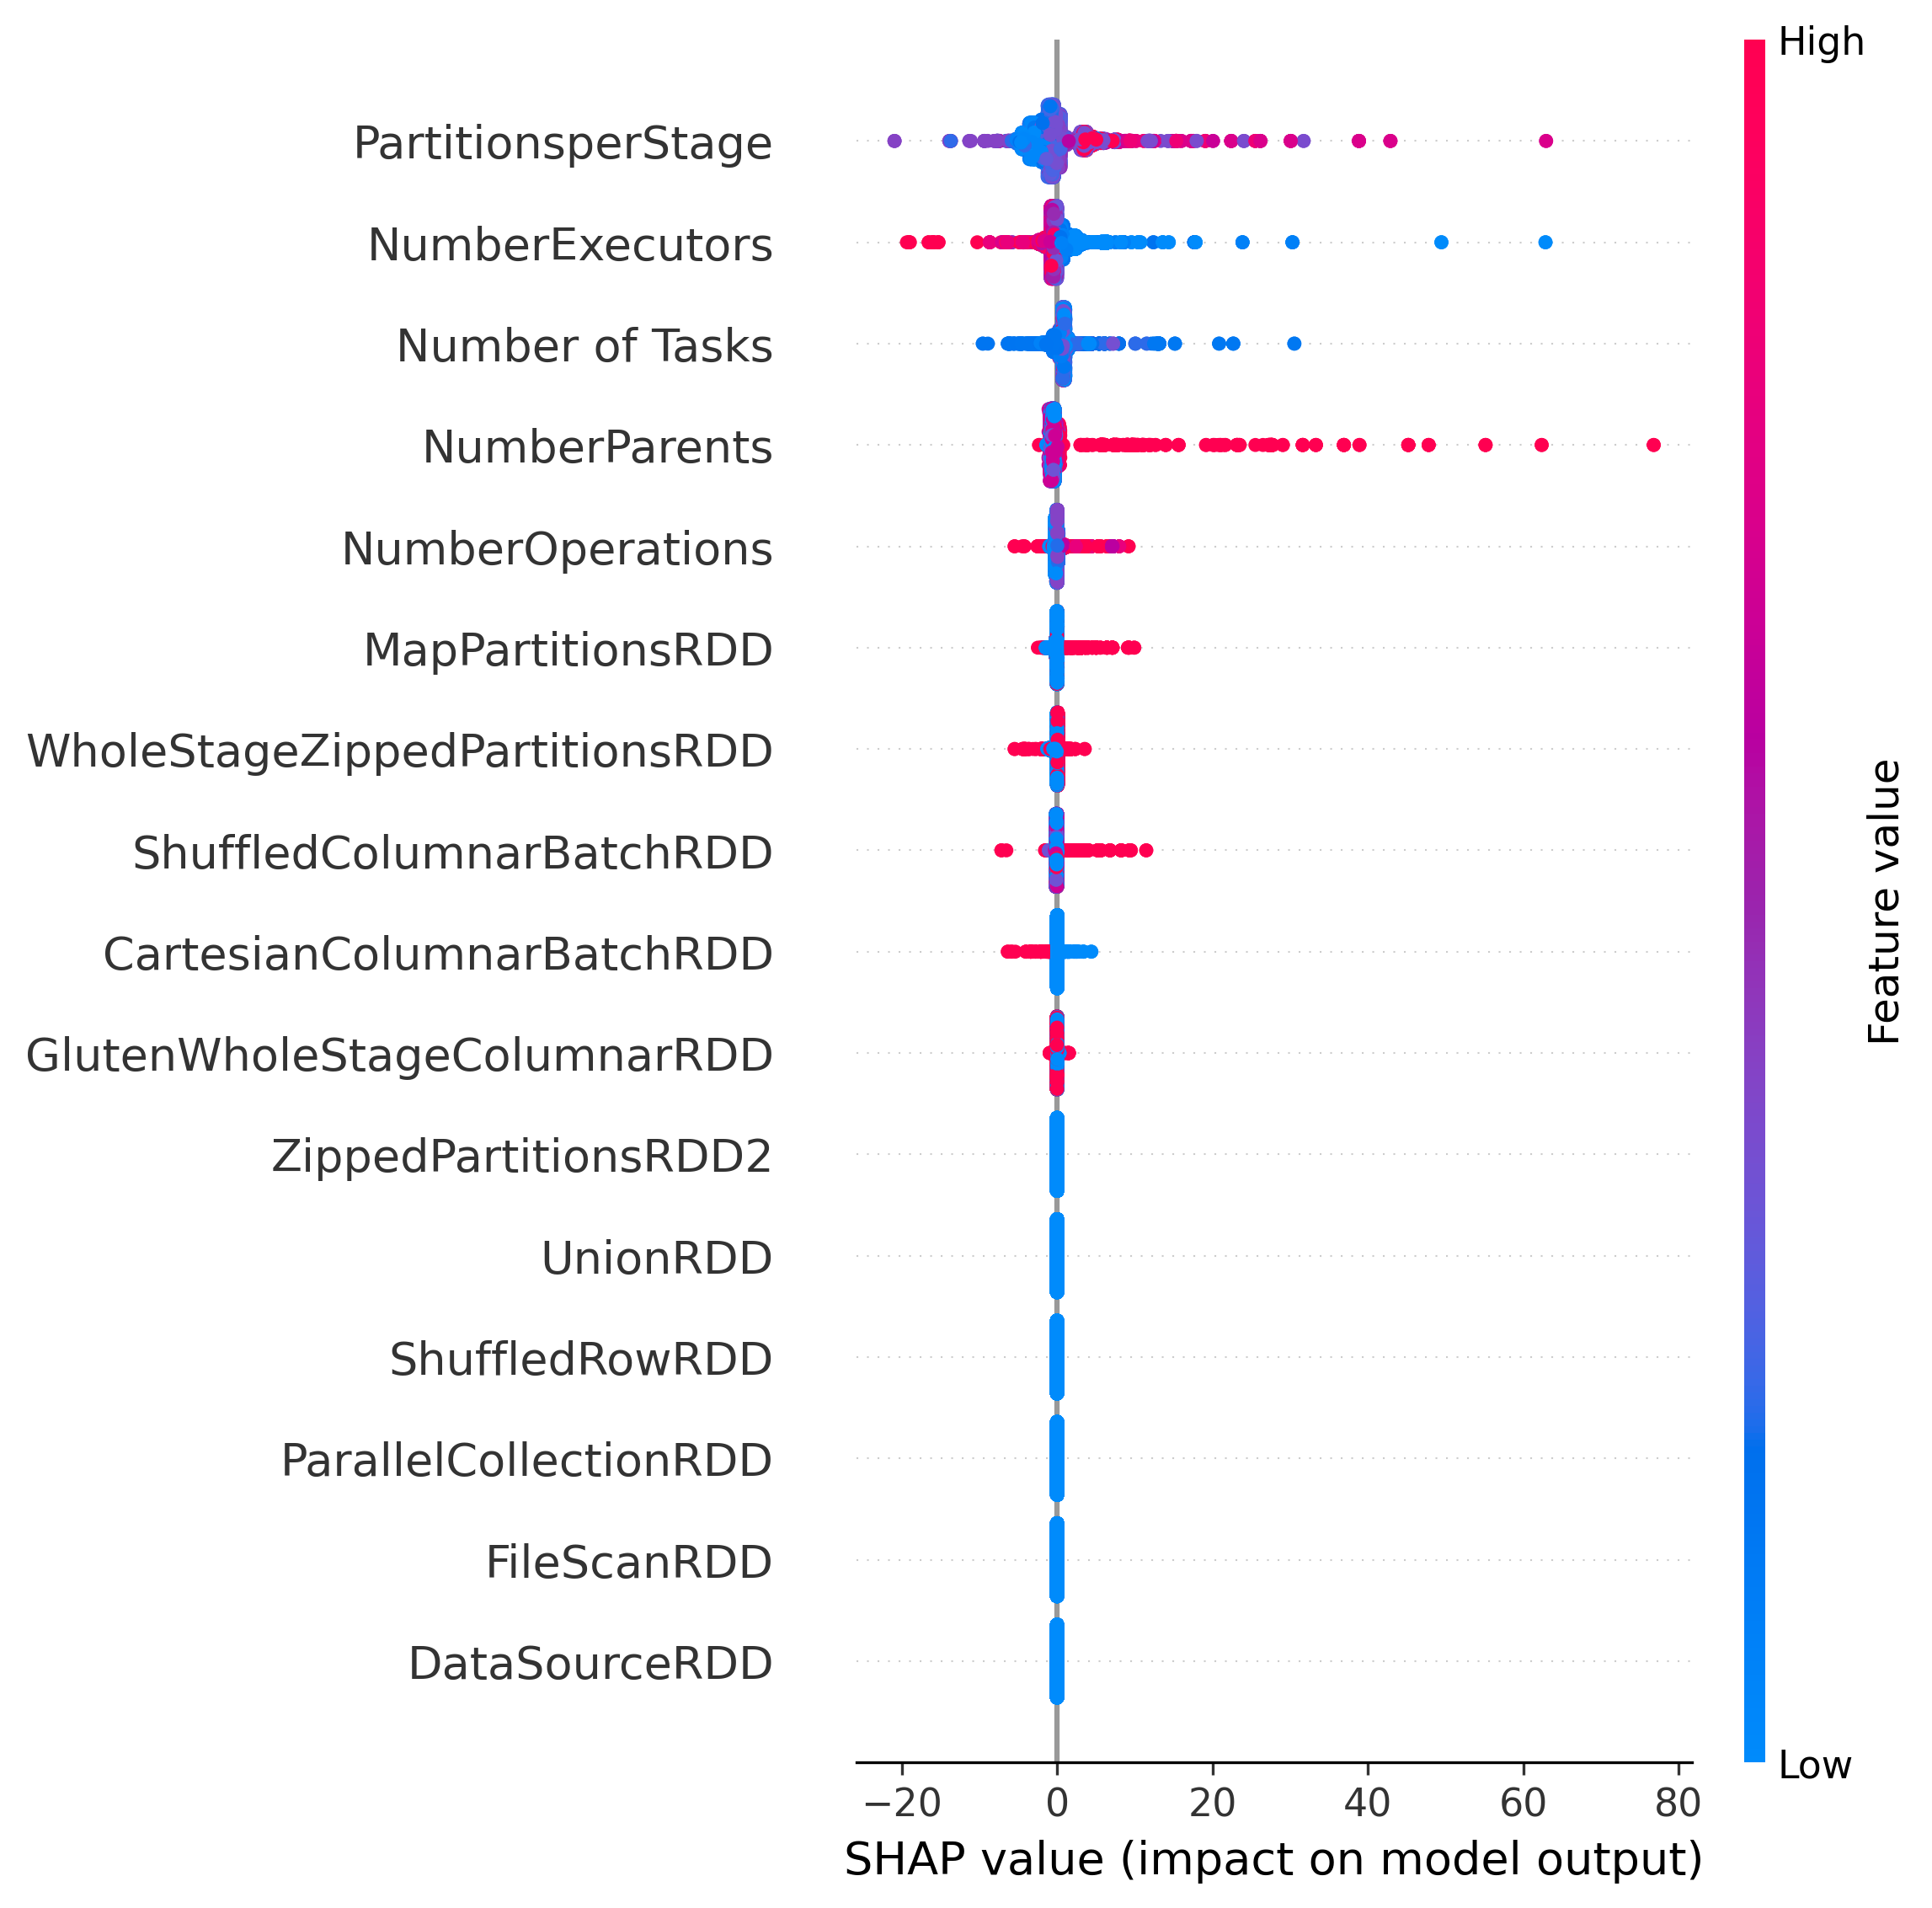
\includegraphics[width=\textwidth]{figs/predictor_shap_beeswarm_SQLStorm_ExecutorRunTimeMaxbyCore_log-True_online.png}
\caption{SQLStorm SHAP Plot 0-shot Cost Predictor}
\label{fig:sqlstorm-shap-0shot}
\end{figure}

\subsubsection{n-shot model}

\begin{figure}[h]
\centering
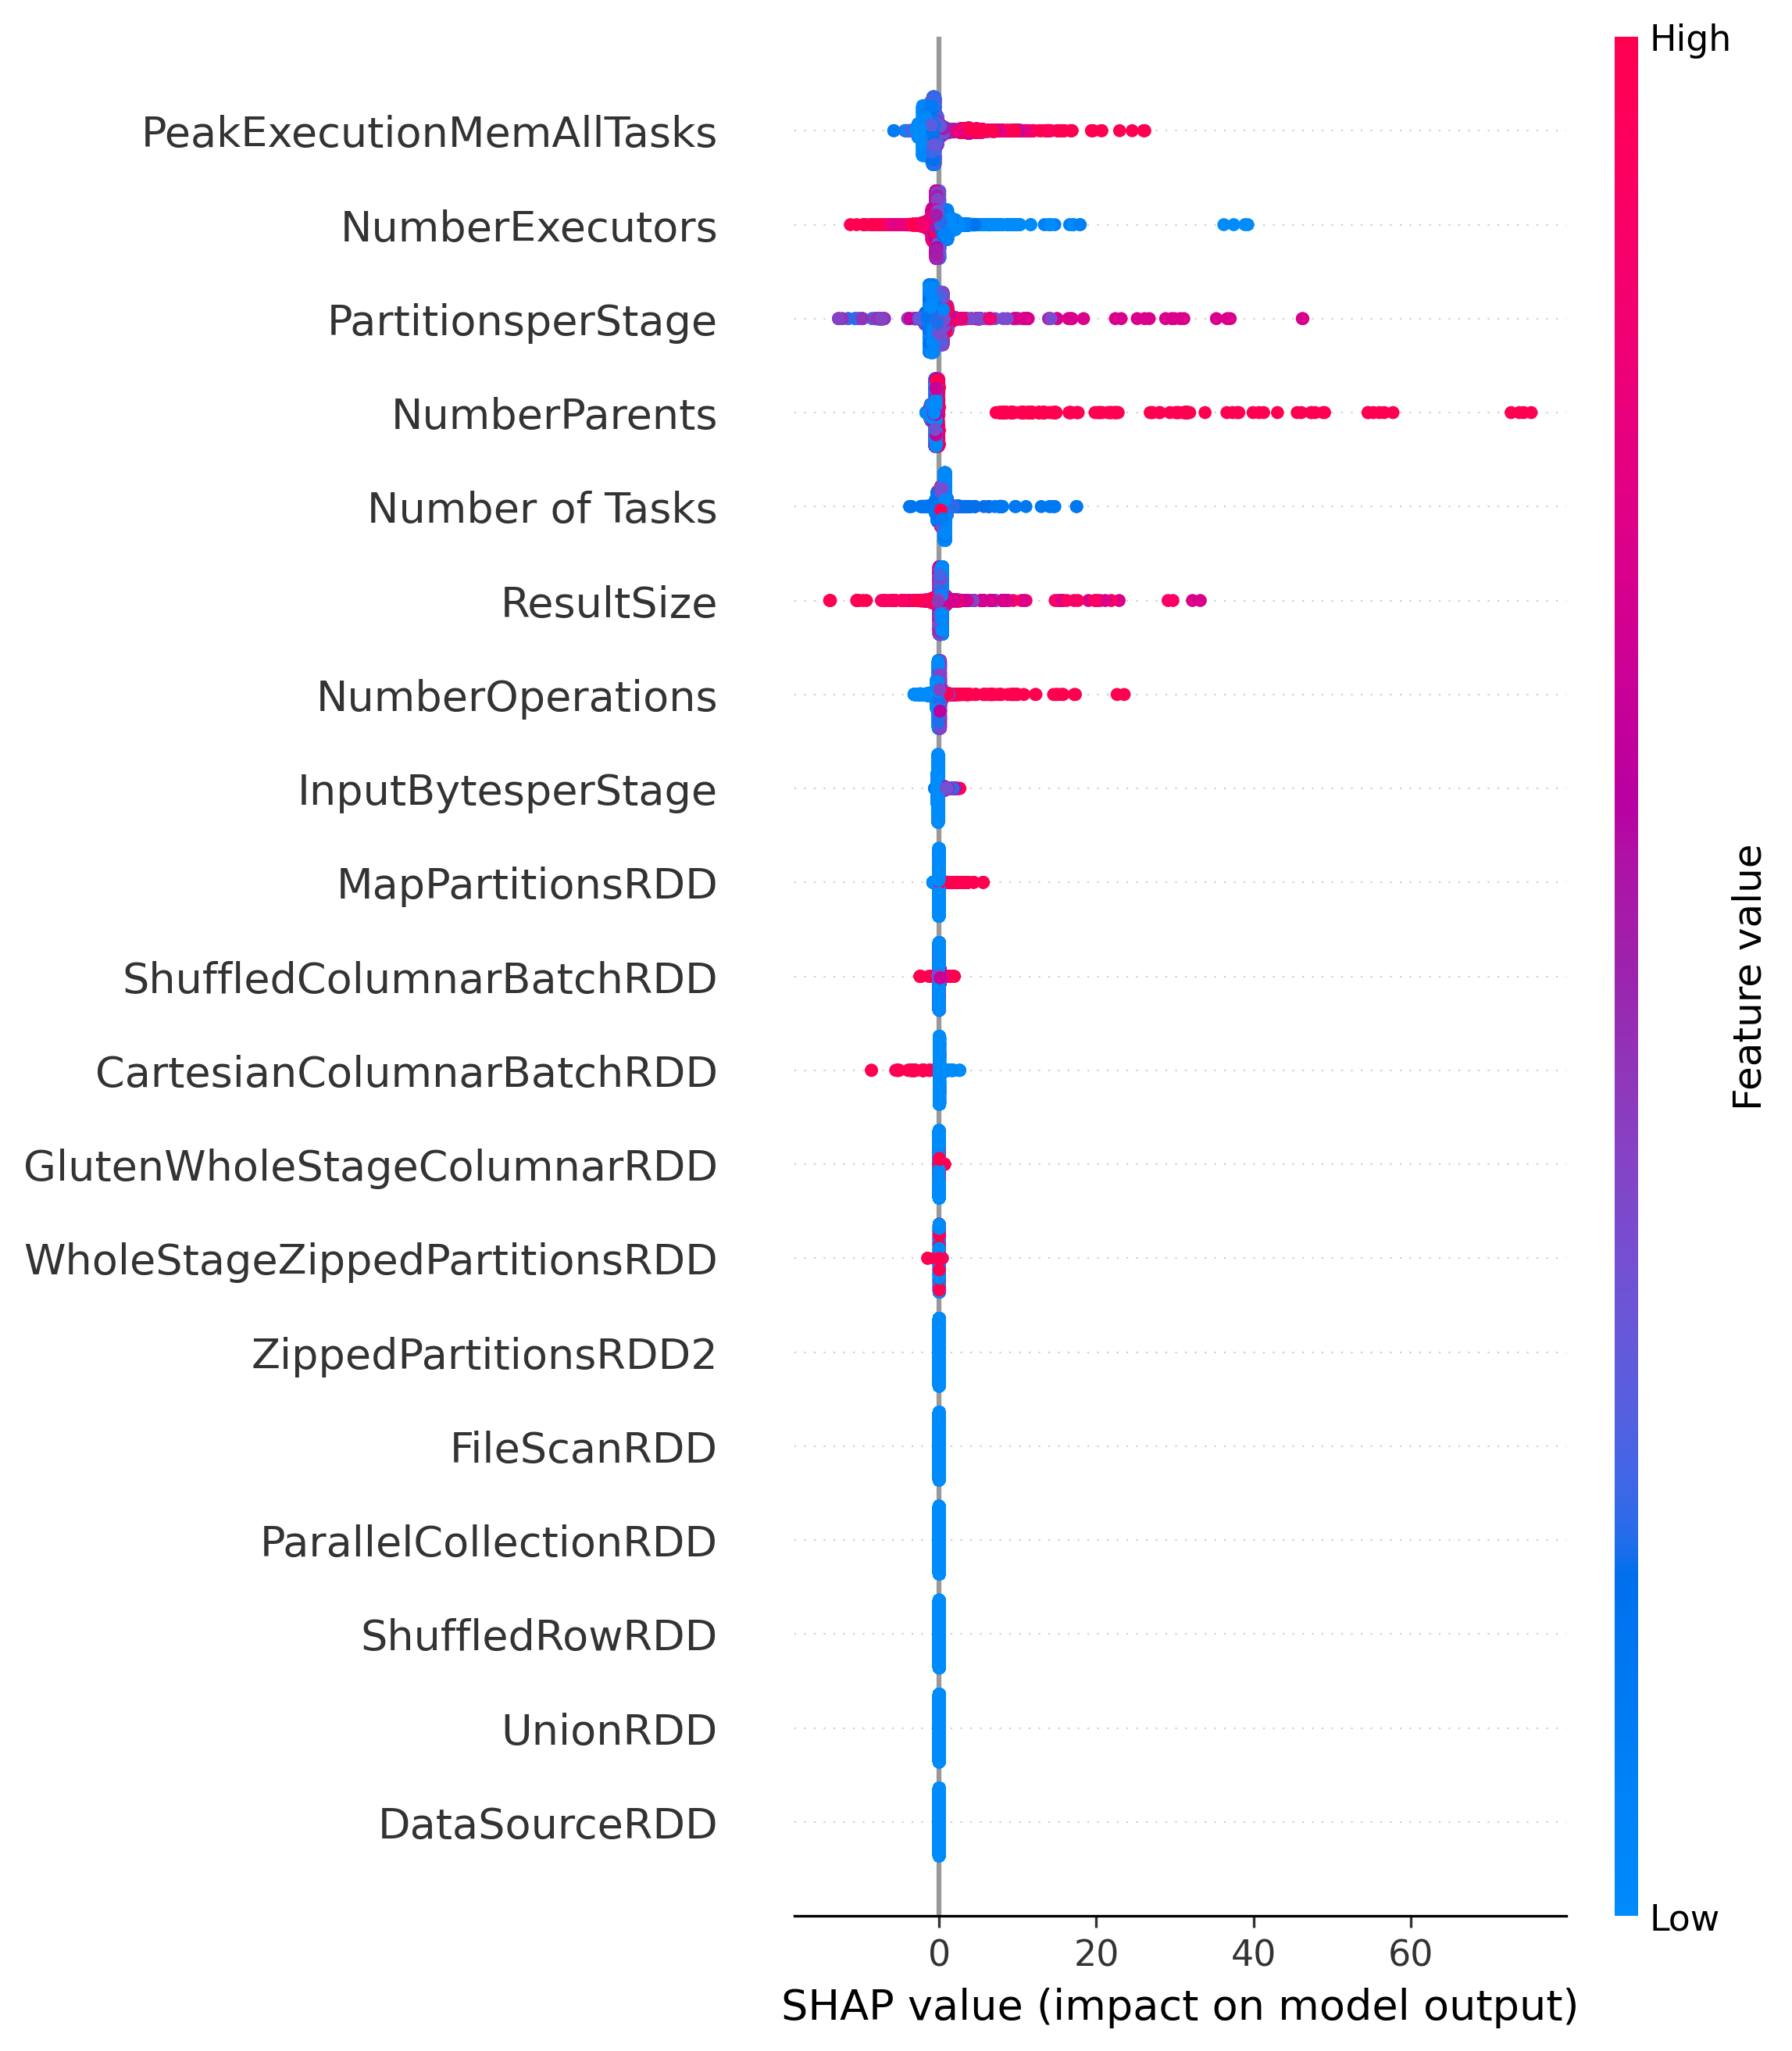
\includegraphics[width=\textwidth]{figs/predictor_shap_beeswarm_SQLStorm_ExecutorRunTimeMaxbyCore_log-True_offline.png}
\caption{SQLStorm SHAP Plot n-shot Cost Predictor}
\label{fig:sqlstorm-shap-nshot}
\end{figure}

\section{Target analyses}

Additional results of end-to-end testing Scenario $\gamma$ using models that predict DurationStage.

\subsection{TPC-DS}

\begin{figure}[h]
\centering
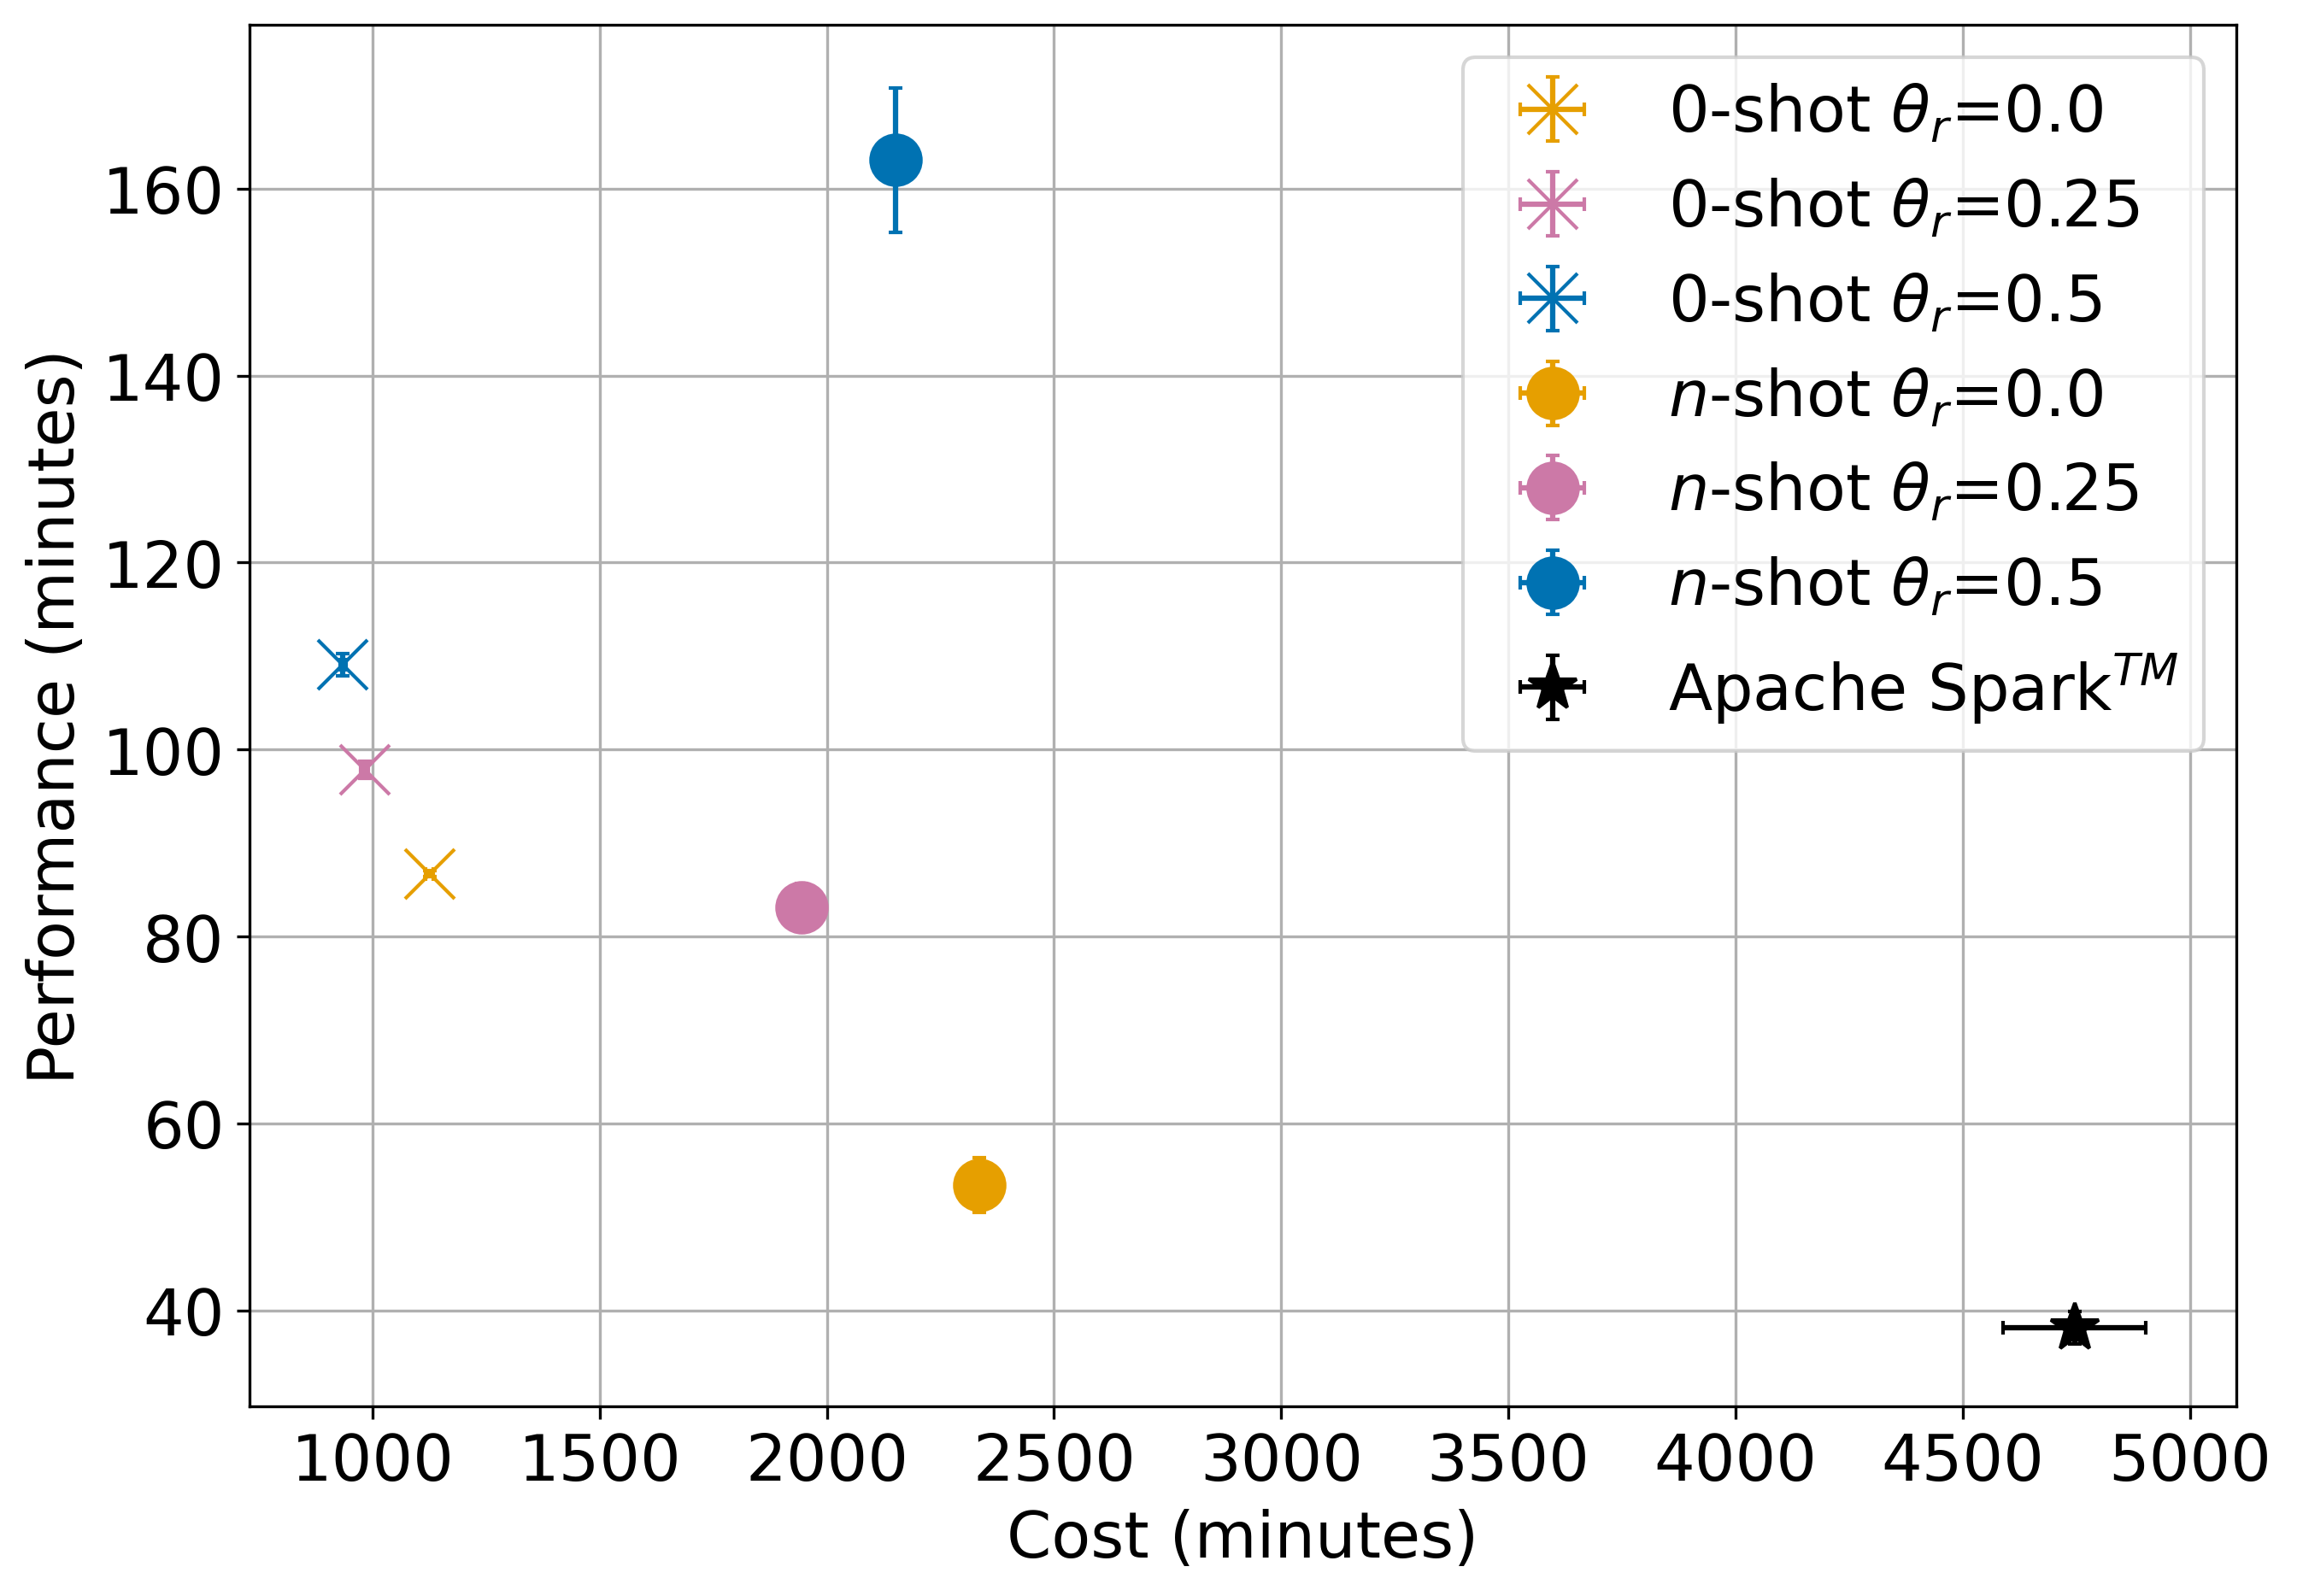
\includegraphics[width=\textwidth]{figs/perfvscost_results_tpcds_duration_target.png}
\caption{TPC-DS Cost and Performance with DurationStage as target}
\label{fig:tpcds-duration-target}
\end{figure}

\subsection{SQLStorm}

\begin{figure}[h]
\centering
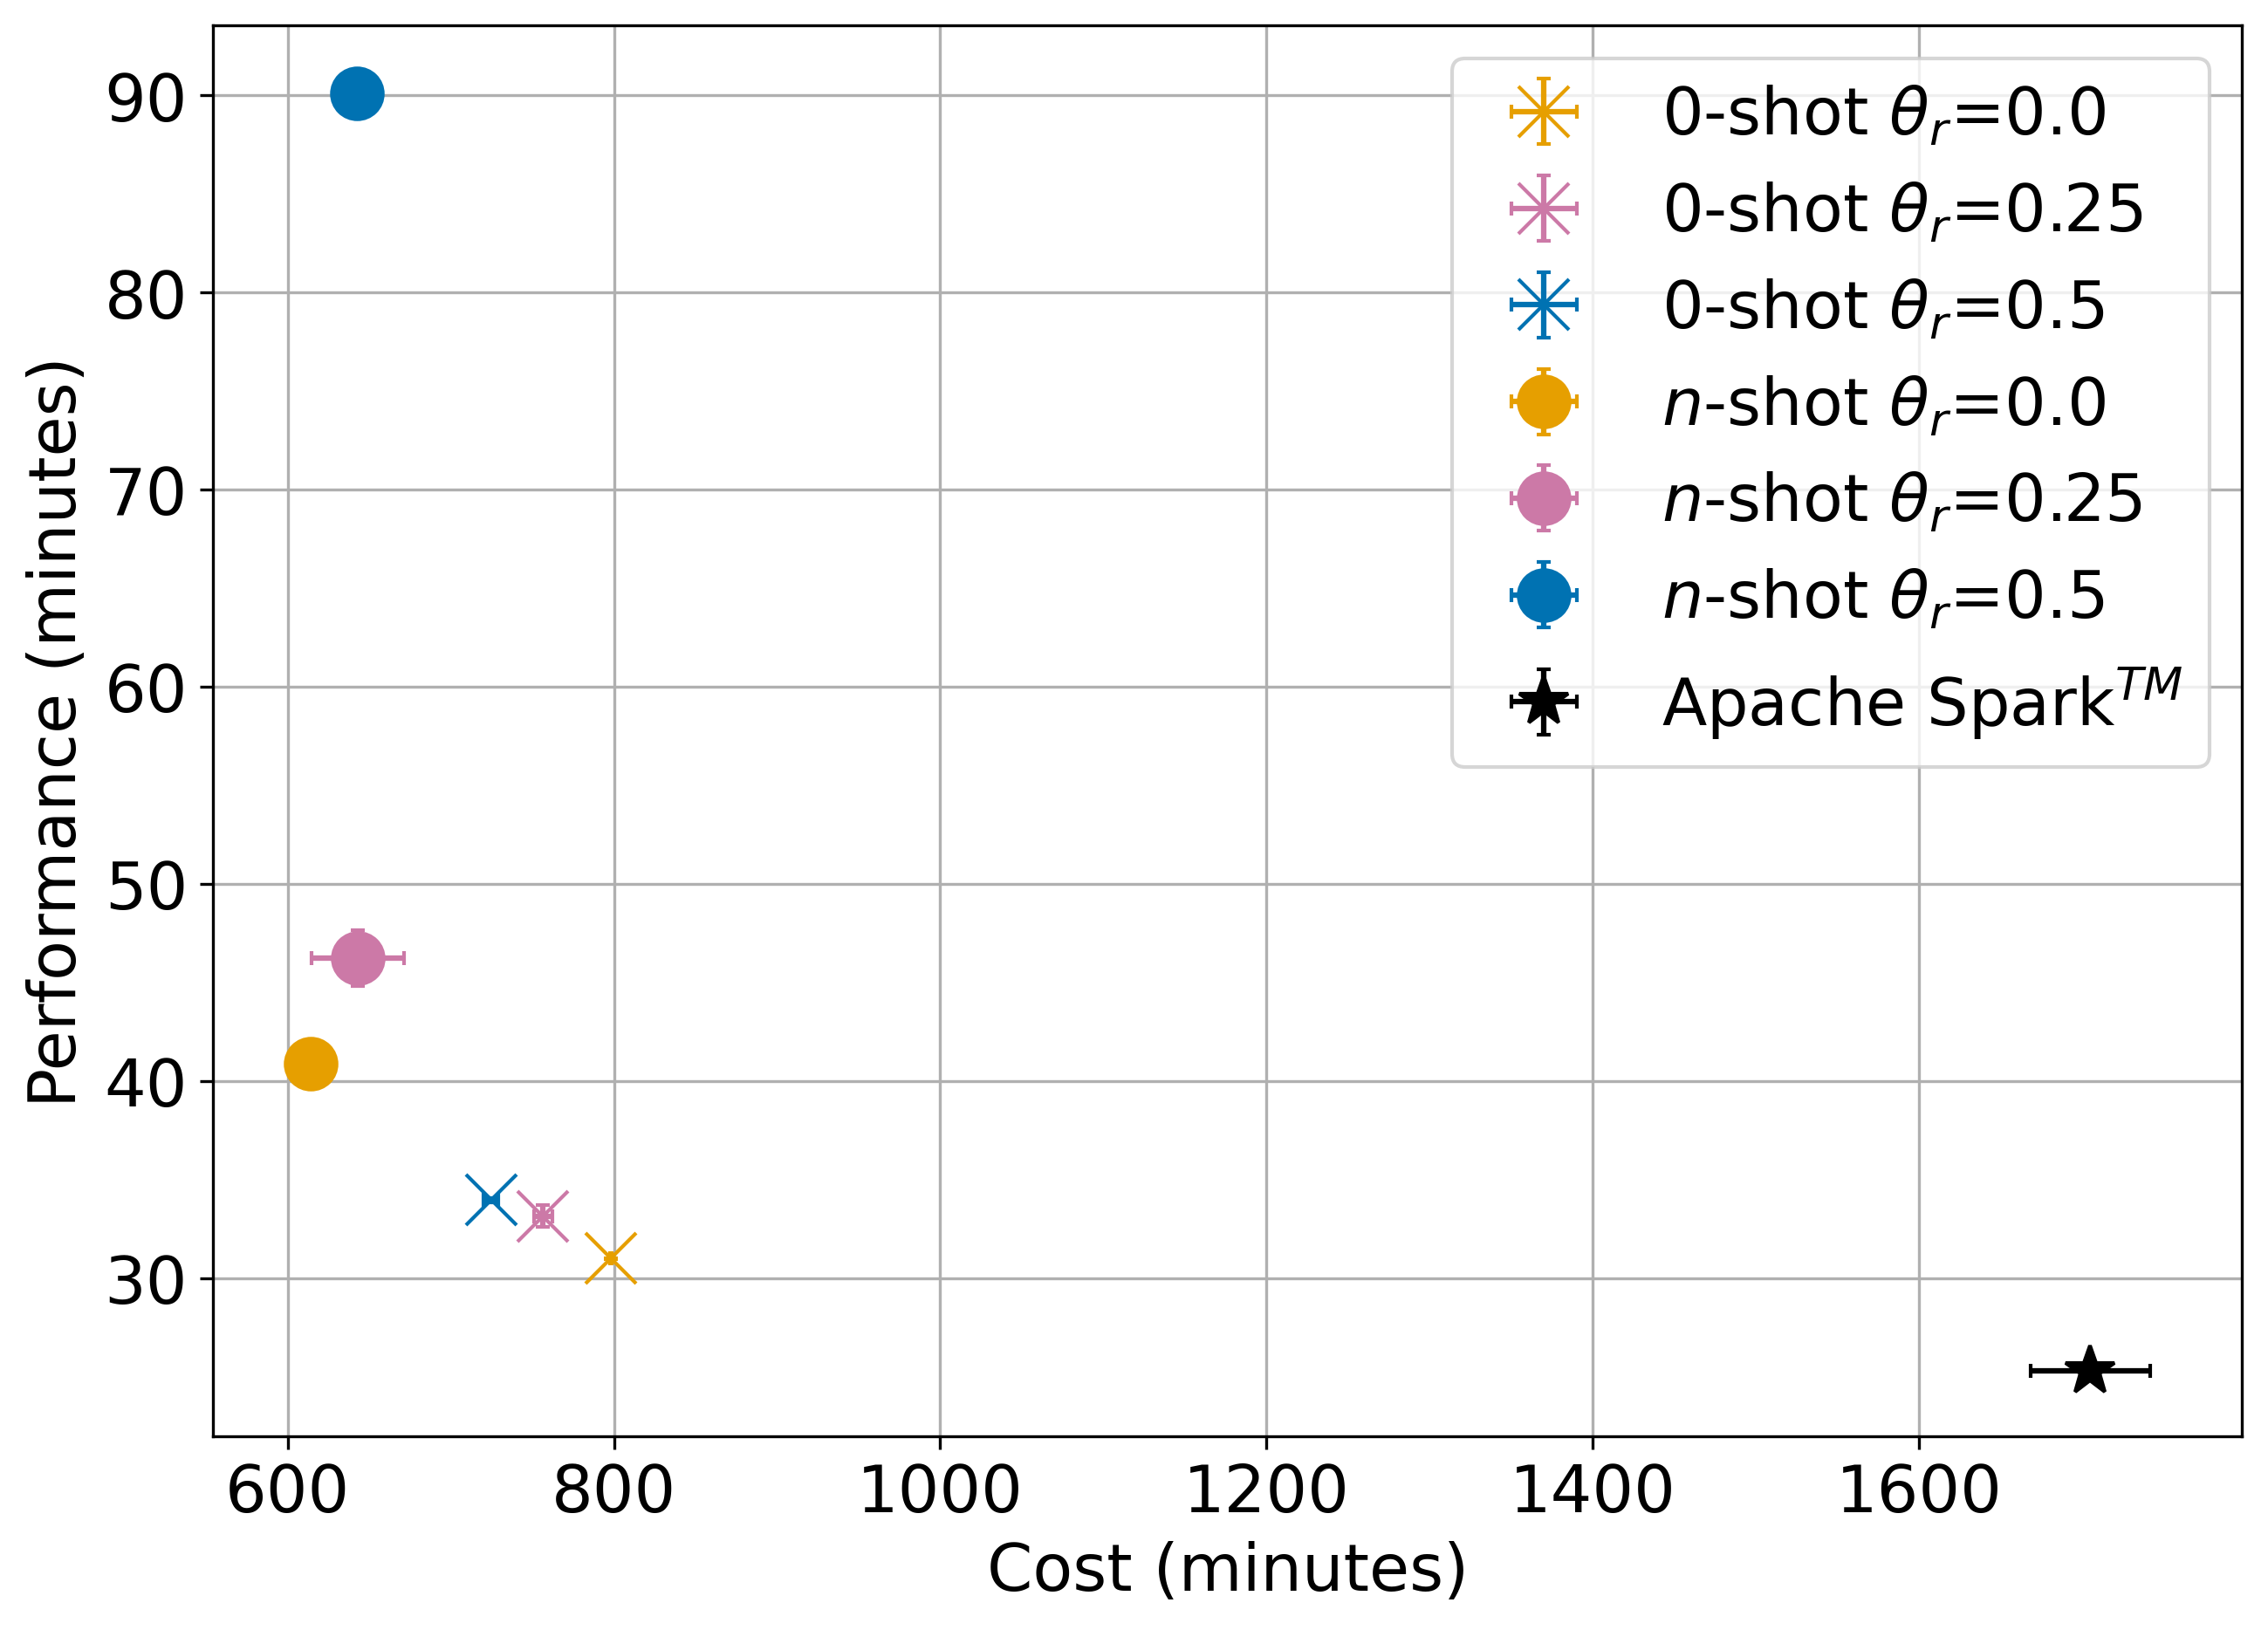
\includegraphics[width=\textwidth]{figs/perfvscost_resultssqlstorm_duration_target.png}
\caption{SQLStorm Cost and Performance with DurationStage as target}
\label{fig:sqlstorm-duration-target}
\end{figure}

\section{Extended Per Query Results}

Additional results on the per query analyses in both benchmarks.

\subsection{TPC-DS}

Radar plots showing Cost and Performance across all queries.

\begin{figure}[h]
\centering
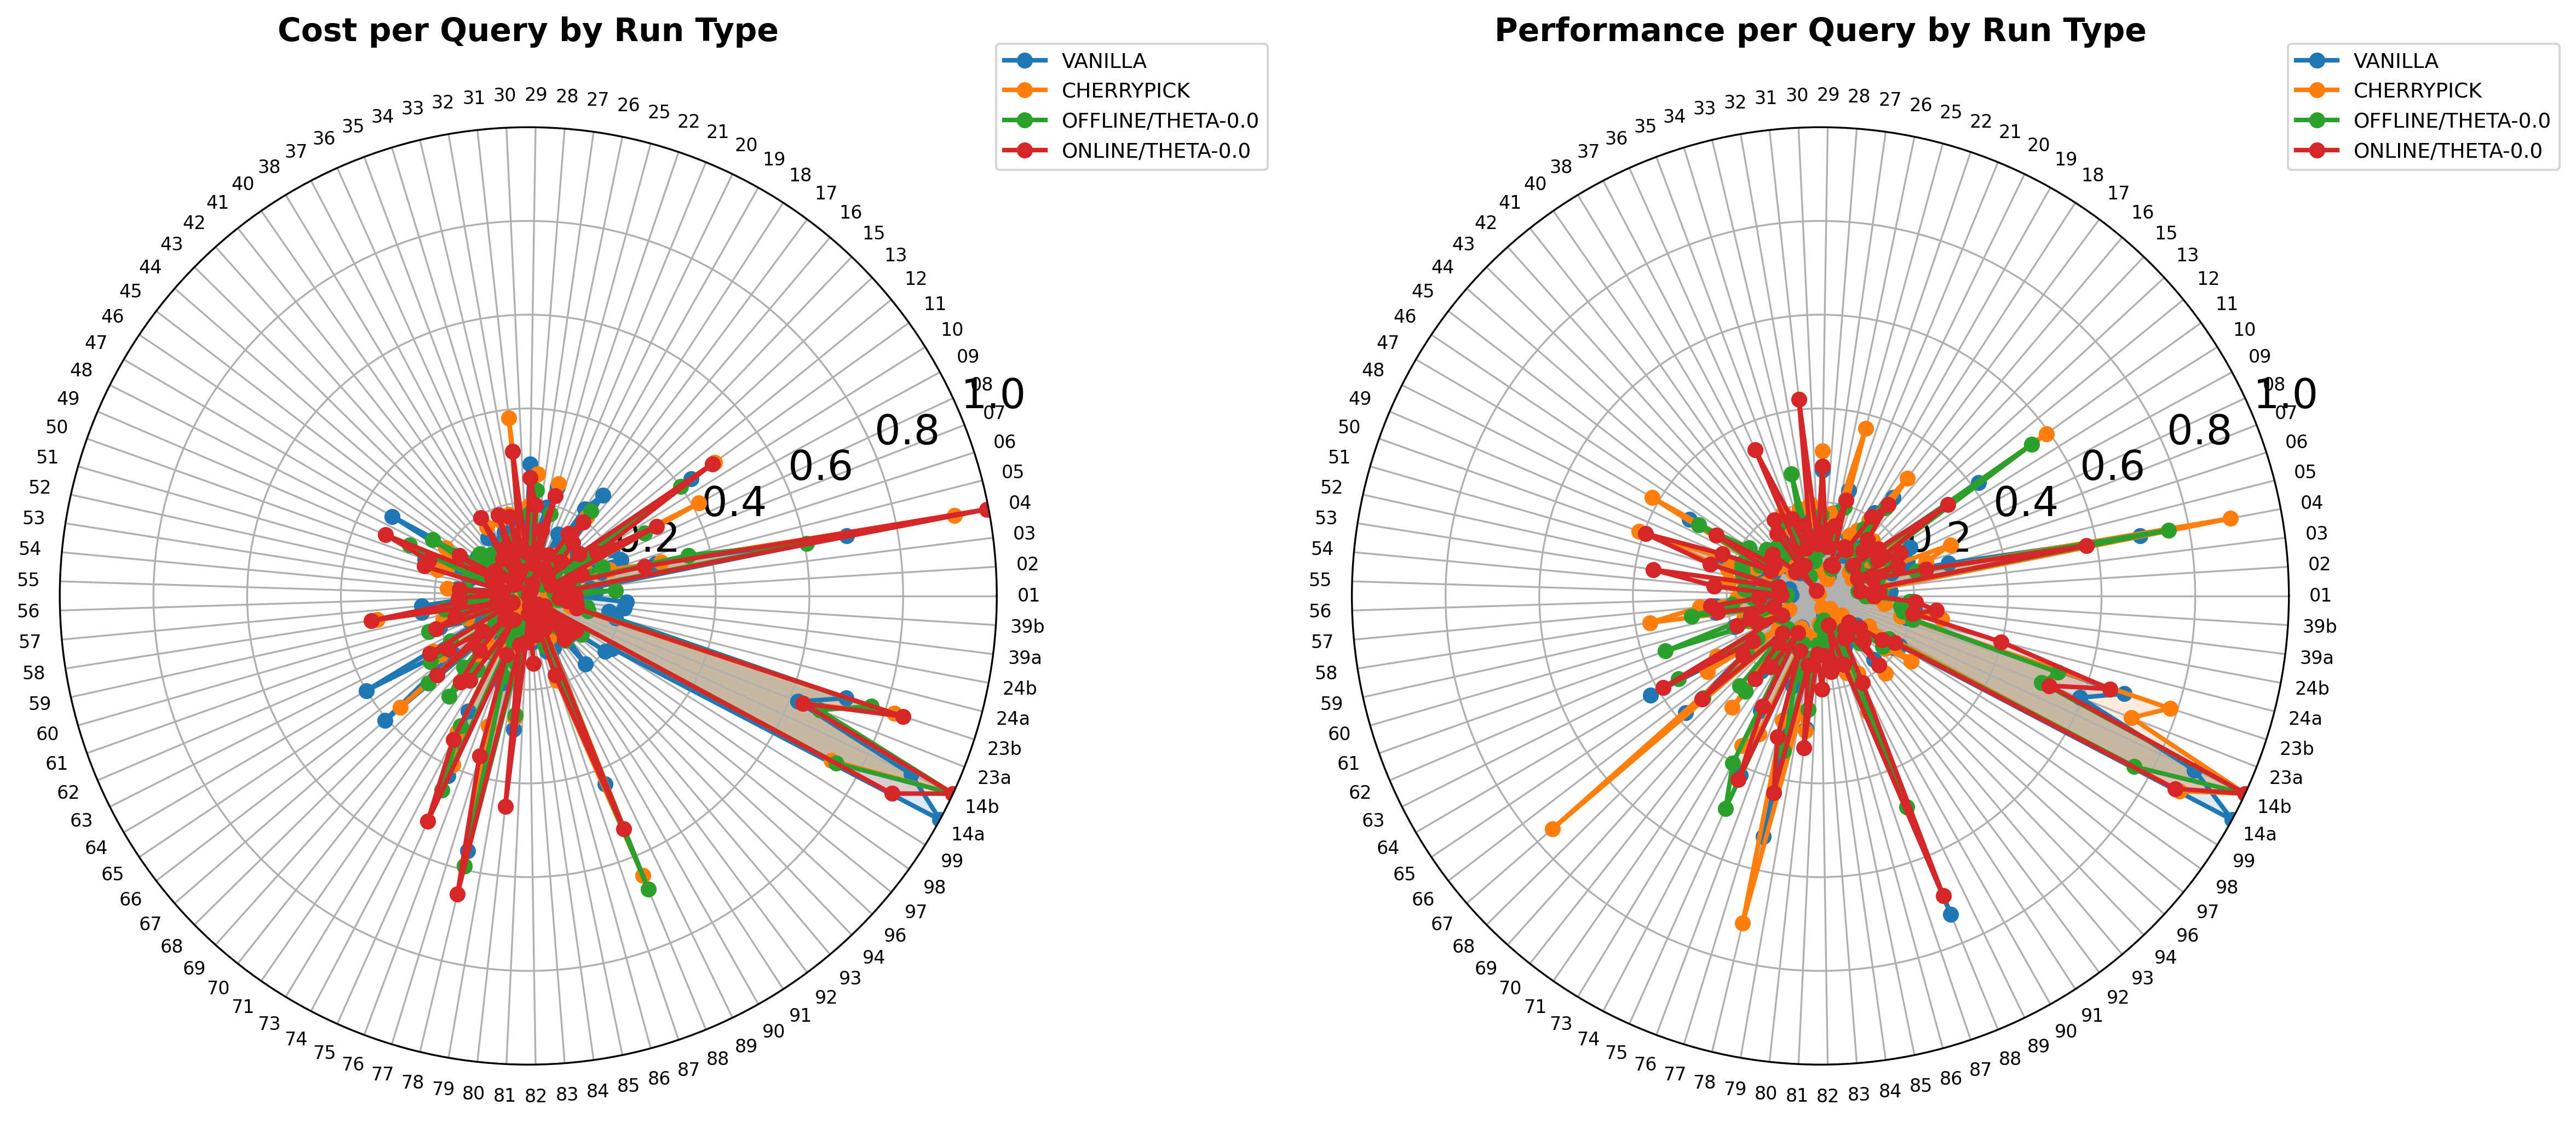
\includegraphics[width=\textwidth]{figs/radar_charts_cost_perf_tpcds.png}
\caption{TPC-DS Radar Charts Cost and Performance}
\label{fig:tpcds-radar}
\end{figure}

The following table shows the top-5 queries with the largest divergence in cost from $0$-shot and Apache Spark approach for TPC-DS.

\begin{table}[h]
\centering
\begin{tabular}{@{}lrrr@{}}
\toprule
\textbf{Query} & \textbf{Cost 0-shot} & \textbf{Cost Apache Spark} & \textbf{Cost Difference} \\
\midrule
14b & 7,209,175 & 16,333,383 & 9,124,208 \\
03 & 528,223 & 9,253,531 & 8,725,308 \\
14a & 6,705,714 & 14,700,672 & 7,994,958 \\
23b & 5,357,945 & 9,911,296 & 4,553,351 \\
04 & 6,476,707 & 10,448,988 & 3,972,281 \\
\bottomrule
\end{tabular}
\caption{Top-5 queries with largest cost divergence for TPC-DS}
\label{tab:tpcds-top5}
\end{table}

\subsection{SQLStorm}

Radar plots showing Cost and Performance across all queries.

\begin{figure}[h]
\centering
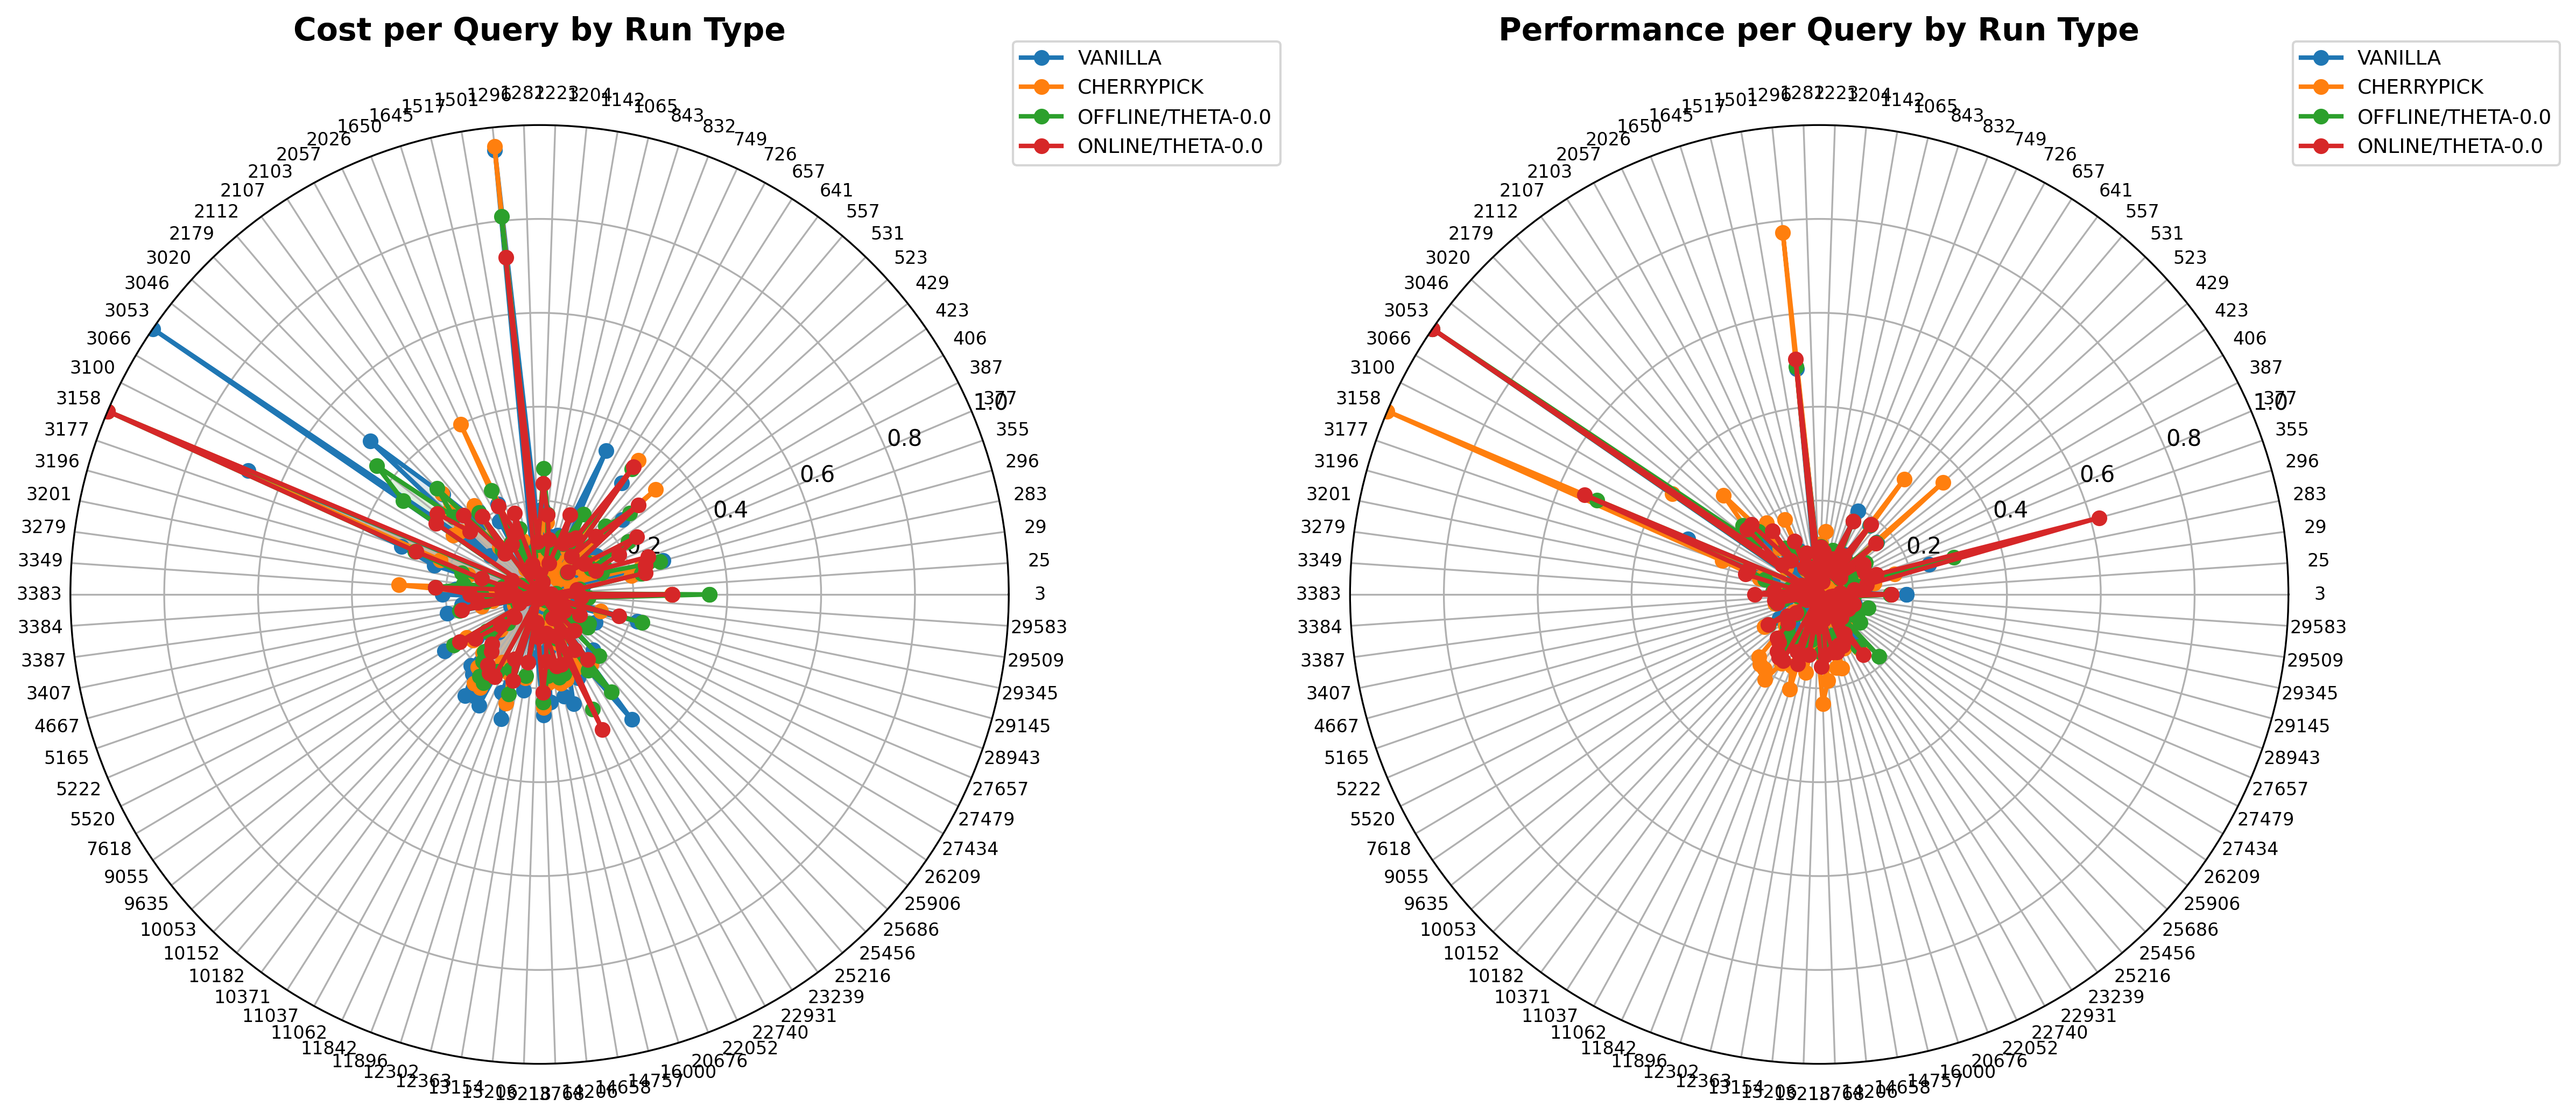
\includegraphics[width=\textwidth]{figs/radar_charts_cost_perf_sqlstorm.png}
\caption{StormSQL Radar Charts Cost and Performance}
\label{fig:sqlstorm-radar}
\end{figure}

The following table shows the top-5 queries with the largest divergence in cost from $0$-shot and Apache Spark approach for SQLStorm.

\begin{table}[h]
\centering
\begin{tabular}{@{}lrrr@{}}
\toprule
\textbf{Query} & \textbf{Cost 0-shot} & \textbf{Cost Apache Spark} & \textbf{Cost Difference} \\
\midrule
3053 & 1,416,380 & 5,810,624 & 4,394,244 \\
1296 & 3,088,394 & 5,723,702 & 2,635,308 \\
3020 & 910,406 & 3,111,072 & 2,200,666 \\
23239 & 694,750 & 2,267,374 & 1,572,624 \\
749 & 561,207 & 1,674,908 & 1,113,701 \\
\bottomrule
\end{tabular}
\caption{Top-5 queries with largest cost divergence for SQLStorm}
\label{tab:sqlstorm-top5}
\end{table}

Furthermore we show cost and performance across all approaches in the top-5 queries for SQLStorm:

\begin{figure}[h]
\centering
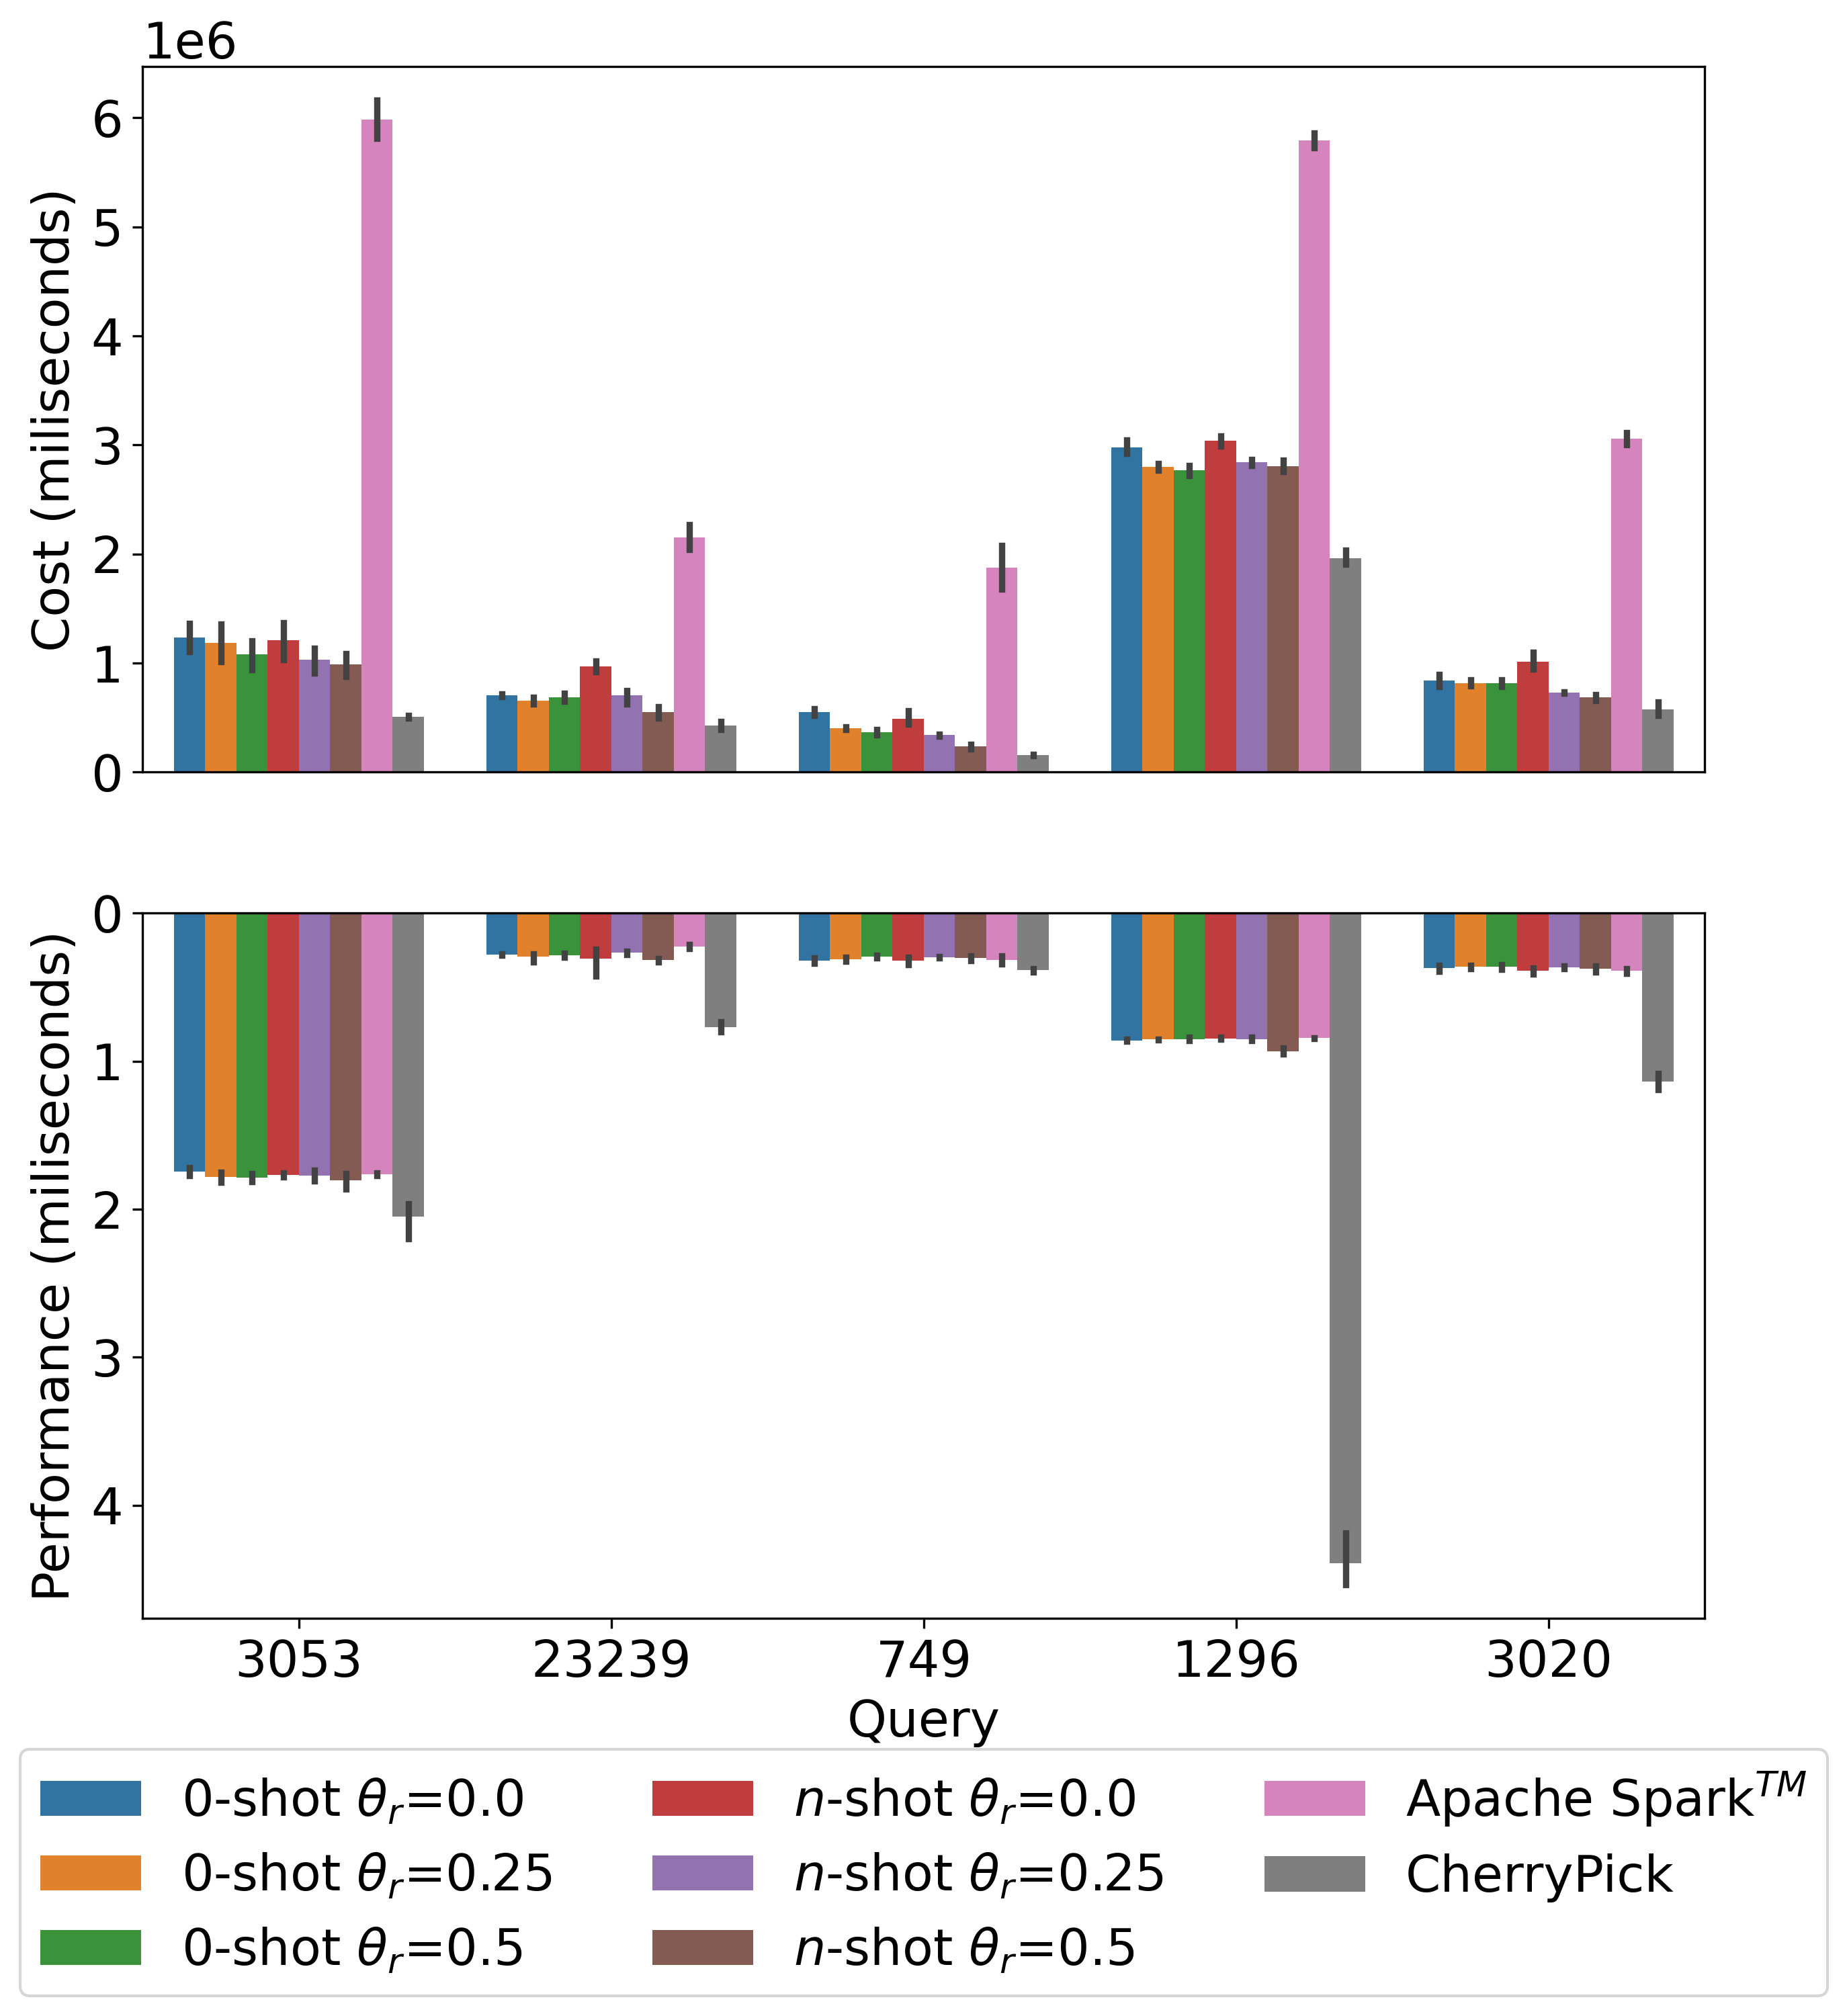
\includegraphics[width=\textwidth]{figs/cost_and_perf_stacked_sqlstorm.png}
\caption{StormSQL top-5 bar plots Cost and Performance}
\label{fig:sqlstorm-top5-bars}
\end{figure}

\section{Data Resources}

The files \texttt{data/performance\_cost\_values\_tcpds\_baselines\_offline\_online\_duration\_final.csv} and \texttt{data/performance\_cost\_values\_tcpds\_baselines\_offline\_online\_maxbycore\_final.csv} contain aggregated statistical summaries of performance and cost metrics for the TPC-DS benchmark comparing different strategies. Columns provide mean and standard deviation values for both Performance (Perf. mean, Perf. std) and Cost (Cost mean, Cost std) metrics across multiple query executions. The dataset includes six optimization strategies: $0$-shot approaches with varying theta parameters ($\theta_r=0.0$, 0.25, and 0.5), three $n$-shot approaches with corresponding theta settings ($\theta_r=0.0$, 0.25, and 0.5), and the Apache Spark baseline for comparison.

The file \texttt{data/performance\_stormsql\_maxbycore\_per\_query.csv} contains performance and cost metrics for the StormSQL benchmark across multiple proposed methods and baseline strategies. Each record includes four key metrics: Performance (Perf.), Cost, both in milliseconds, Query identifier, and method (optimization strategy). The dataset encompasses multiple run methods including ONLINE/THETA-0.0, ONLINE/THETA-0.25, ONLINE/THETA-0.5, OFFLINE/THETA-0.0, OFFLINE/THETA-0.25, OFFLINE/THETA-0.5, VANILLA baseline, and CHERRY-PICK strategies. Where ONLINE = $0$-shot approach, OFFLINE = $n$-shot approach, VANILLA = Apache Spark run. The data represents multiple executions per query (indicated by repeated Query IDs with varying Perf. and Cost values), allowing for analysis of performance variability and consistency across different approaches. Similarly \texttt{data/performance\_tpcds\_maxbycore\_per\_query.csv} contains same metrics for TPC-DS.

% Made with Bob
